\documentclass{standalone}
\usepackage{tikz}
\usetikzlibrary{positioning}

\begin{document}
  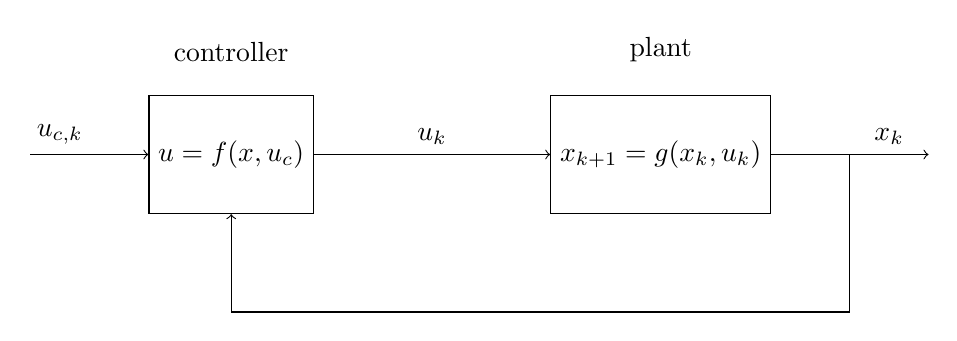
\begin{tikzpicture}[block/.style={rectangle, draw, minimum height=15mm, minimum width=20mm},
    ]
    \node[block] (controller) {$u = f(x, u_{c})$};
    \node[block, right=3cm of controller] (plant) {$x_{k+1} = g(x_k, u_k)$};
    \node[coordinate, left = 15mm of controller] (input) {};
    \node[coordinate, right = 10mm of plant] (measure) {};
    \node[coordinate, right = 10mm of measure] (output) {};

    \node[above = 0.3cm of controller] {controller};
    \node[above = 0.3cm of plant] {plant};

    \draw[->] (input) -- node[above, near start] {$u_{c,k}$} (controller);
    \draw[->] (plant) -- node[above, near end] {$x_{k}$} (output);
    \draw[->] (measure) -- ++(0,-20mm) -| (controller);
    \draw[->] (controller) -- node[above, ] {$u_{k}$} (plant);
  \end{tikzpicture}
\end{document}
